% Options for packages loaded elsewhere
\PassOptionsToPackage{unicode}{hyperref}
\PassOptionsToPackage{hyphens}{url}
%
\documentclass[
  ignorenonframetext,
]{beamer}
\usepackage{pgfpages}
\setbeamertemplate{caption}[numbered]
\setbeamertemplate{caption label separator}{: }
\setbeamercolor{caption name}{fg=normal text.fg}
\beamertemplatenavigationsymbolsempty
% Prevent slide breaks in the middle of a paragraph
\widowpenalties 1 10000
\raggedbottom
\setbeamertemplate{part page}{
  \centering
  \begin{beamercolorbox}[sep=16pt,center]{part title}
    \usebeamerfont{part title}\insertpart\par
  \end{beamercolorbox}
}
\setbeamertemplate{section page}{
  \centering
  \begin{beamercolorbox}[sep=12pt,center]{part title}
    \usebeamerfont{section title}\insertsection\par
  \end{beamercolorbox}
}
\setbeamertemplate{subsection page}{
  \centering
  \begin{beamercolorbox}[sep=8pt,center]{part title}
    \usebeamerfont{subsection title}\insertsubsection\par
  \end{beamercolorbox}
}
\AtBeginPart{
  \frame{\partpage}
}
\AtBeginSection{
  \ifbibliography
  \else
    \frame{\sectionpage}
  \fi
}
\AtBeginSubsection{
  \frame{\subsectionpage}
}
\usepackage{amsmath,amssymb}
\usepackage{iftex}
\ifPDFTeX
  \usepackage[T1]{fontenc}
  \usepackage[utf8]{inputenc}
  \usepackage{textcomp} % provide euro and other symbols
\else % if luatex or xetex
  \usepackage{unicode-math} % this also loads fontspec
  \defaultfontfeatures{Scale=MatchLowercase}
  \defaultfontfeatures[\rmfamily]{Ligatures=TeX,Scale=1}
\fi
\usepackage{lmodern}
\usetheme[]{Boadilla}
\ifPDFTeX\else
  % xetex/luatex font selection
\fi
% Use upquote if available, for straight quotes in verbatim environments
\IfFileExists{upquote.sty}{\usepackage{upquote}}{}
\IfFileExists{microtype.sty}{% use microtype if available
  \usepackage[]{microtype}
  \UseMicrotypeSet[protrusion]{basicmath} % disable protrusion for tt fonts
}{}
\makeatletter
\@ifundefined{KOMAClassName}{% if non-KOMA class
  \IfFileExists{parskip.sty}{%
    \usepackage{parskip}
  }{% else
    \setlength{\parindent}{0pt}
    \setlength{\parskip}{6pt plus 2pt minus 1pt}}
}{% if KOMA class
  \KOMAoptions{parskip=half}}
\makeatother
\usepackage{xcolor}
\newif\ifbibliography
\usepackage{color}
\usepackage{fancyvrb}
\newcommand{\VerbBar}{|}
\newcommand{\VERB}{\Verb[commandchars=\\\{\}]}
\DefineVerbatimEnvironment{Highlighting}{Verbatim}{commandchars=\\\{\}}
% Add ',fontsize=\small' for more characters per line
\usepackage{framed}
\definecolor{shadecolor}{RGB}{248,248,248}
\newenvironment{Shaded}{\begin{snugshade}}{\end{snugshade}}
\newcommand{\AlertTok}[1]{\textcolor[rgb]{0.94,0.16,0.16}{#1}}
\newcommand{\AnnotationTok}[1]{\textcolor[rgb]{0.56,0.35,0.01}{\textbf{\textit{#1}}}}
\newcommand{\AttributeTok}[1]{\textcolor[rgb]{0.13,0.29,0.53}{#1}}
\newcommand{\BaseNTok}[1]{\textcolor[rgb]{0.00,0.00,0.81}{#1}}
\newcommand{\BuiltInTok}[1]{#1}
\newcommand{\CharTok}[1]{\textcolor[rgb]{0.31,0.60,0.02}{#1}}
\newcommand{\CommentTok}[1]{\textcolor[rgb]{0.56,0.35,0.01}{\textit{#1}}}
\newcommand{\CommentVarTok}[1]{\textcolor[rgb]{0.56,0.35,0.01}{\textbf{\textit{#1}}}}
\newcommand{\ConstantTok}[1]{\textcolor[rgb]{0.56,0.35,0.01}{#1}}
\newcommand{\ControlFlowTok}[1]{\textcolor[rgb]{0.13,0.29,0.53}{\textbf{#1}}}
\newcommand{\DataTypeTok}[1]{\textcolor[rgb]{0.13,0.29,0.53}{#1}}
\newcommand{\DecValTok}[1]{\textcolor[rgb]{0.00,0.00,0.81}{#1}}
\newcommand{\DocumentationTok}[1]{\textcolor[rgb]{0.56,0.35,0.01}{\textbf{\textit{#1}}}}
\newcommand{\ErrorTok}[1]{\textcolor[rgb]{0.64,0.00,0.00}{\textbf{#1}}}
\newcommand{\ExtensionTok}[1]{#1}
\newcommand{\FloatTok}[1]{\textcolor[rgb]{0.00,0.00,0.81}{#1}}
\newcommand{\FunctionTok}[1]{\textcolor[rgb]{0.13,0.29,0.53}{\textbf{#1}}}
\newcommand{\ImportTok}[1]{#1}
\newcommand{\InformationTok}[1]{\textcolor[rgb]{0.56,0.35,0.01}{\textbf{\textit{#1}}}}
\newcommand{\KeywordTok}[1]{\textcolor[rgb]{0.13,0.29,0.53}{\textbf{#1}}}
\newcommand{\NormalTok}[1]{#1}
\newcommand{\OperatorTok}[1]{\textcolor[rgb]{0.81,0.36,0.00}{\textbf{#1}}}
\newcommand{\OtherTok}[1]{\textcolor[rgb]{0.56,0.35,0.01}{#1}}
\newcommand{\PreprocessorTok}[1]{\textcolor[rgb]{0.56,0.35,0.01}{\textit{#1}}}
\newcommand{\RegionMarkerTok}[1]{#1}
\newcommand{\SpecialCharTok}[1]{\textcolor[rgb]{0.81,0.36,0.00}{\textbf{#1}}}
\newcommand{\SpecialStringTok}[1]{\textcolor[rgb]{0.31,0.60,0.02}{#1}}
\newcommand{\StringTok}[1]{\textcolor[rgb]{0.31,0.60,0.02}{#1}}
\newcommand{\VariableTok}[1]{\textcolor[rgb]{0.00,0.00,0.00}{#1}}
\newcommand{\VerbatimStringTok}[1]{\textcolor[rgb]{0.31,0.60,0.02}{#1}}
\newcommand{\WarningTok}[1]{\textcolor[rgb]{0.56,0.35,0.01}{\textbf{\textit{#1}}}}
\usepackage{longtable,booktabs,array}
\usepackage{calc} % for calculating minipage widths
\usepackage{caption}
% Make caption package work with longtable
\makeatletter
\def\fnum@table{\tablename~\thetable}
\makeatother
\usepackage{graphicx}
\makeatletter
\def\maxwidth{\ifdim\Gin@nat@width>\linewidth\linewidth\else\Gin@nat@width\fi}
\def\maxheight{\ifdim\Gin@nat@height>\textheight\textheight\else\Gin@nat@height\fi}
\makeatother
% Scale images if necessary, so that they will not overflow the page
% margins by default, and it is still possible to overwrite the defaults
% using explicit options in \includegraphics[width, height, ...]{}
\setkeys{Gin}{width=\maxwidth,height=\maxheight,keepaspectratio}
% Set default figure placement to htbp
\makeatletter
\def\fps@figure{htbp}
\makeatother
\setlength{\emergencystretch}{3em} % prevent overfull lines
\providecommand{\tightlist}{%
  \setlength{\itemsep}{0pt}\setlength{\parskip}{0pt}}
\setcounter{secnumdepth}{-\maxdimen} % remove section numbering
\usepackage{graphicx}
\logo{\ifnum\thepage>1\hfill
\includegraphics[width=1cm]{logo}\fi}
\titlegraphic{
\includegraphics[width=3cm]{logo}}
\newcommand{\theHtable}{\thetable}
\ifLuaTeX
  \usepackage{selnolig}  % disable illegal ligatures
\fi
\usepackage{bookmark}
\IfFileExists{xurl.sty}{\usepackage{xurl}}{} % add URL line breaks if available
\urlstyle{same}
\hypersetup{
  pdftitle={Hypothesis Testing, Probability and Distributions},
  pdfauthor={Pablo E. Gutiérrez-Fonseca},
  hidelinks,
  pdfcreator={LaTeX via pandoc}}

\title{Hypothesis Testing, Probability and Distributions}
\author{Pablo E. Gutiérrez-Fonseca}
\date{Fall 2024}

\begin{document}
\frame{\titlepage}

\begin{frame}{Normality, Probability and Significance}
\phantomsection\label{normality-probability-and-significance}
\begin{itemize}
\tightlist
\item
  Why did we focus on normality?

  \begin{itemize}
  \tightlist
  \item
    The \textbf{normal distribution} is a key tool for determining the
    probability of a given value occurring in a population that follows
    this distribution.
  \end{itemize}
\end{itemize}

\begin{itemize}
\tightlist
\item
  It allows us to make inferences about a population by calculating how
  likely it is for data to fall within certain ranges.
\end{itemize}

\begin{itemize}
\tightlist
\item
  Many statistical tests assume data follows a \textbf{normal
  distribution}, which helps in determining \textbf{significance} and
  making reliable conclusions.
\end{itemize}
\end{frame}

\begin{frame}{Hypothesis Testing}
\phantomsection\label{hypothesis-testing}
\begin{itemize}
\tightlist
\item
  All inferential tests use a formula that calculates a \textbf{test
  statistic}, quantifying the relationship or difference you are
  testing.
\end{itemize}
\end{frame}

\begin{frame}{Hypothesis Testing}
\phantomsection\label{hypothesis-testing-1}
\begin{itemize}
\tightlist
\item
  We use the \textbf{normal distribution curve} to find the
  \textbf{probability} of obtaining a \textbf{test statistic} as extreme
  as the one observed, assuming the \textbf{Null Hypothesis is true}.
\end{itemize}
\end{frame}

\begin{frame}{Hypothesis Testing}
\phantomsection\label{hypothesis-testing-2}
\begin{itemize}
\tightlist
\item
  If the \textbf{probability} (\emph{\emph{the area under the curve}})
  of obtaining a test statistic that extreme is less than our chosen
  significance threshold (\emph{\emph{usually 0.05}}), we conclude that
  the result is \textbf{statistically significant}.
\end{itemize}
\end{frame}

\begin{frame}{Hypothesis Testing}
\phantomsection\label{hypothesis-testing-3}
\begin{itemize}
\tightlist
\item
  Another way to think about this:

  \begin{itemize}
  \tightlist
  \item
    If the probability that our data \textbf{fits the null distribution
    (i.e., the null hypothesis is true) is less than 5\%}, then we
    conclude that the data \textbf{does not fit the null}.

    \begin{itemize}
    \tightlist
    \item
      \textbf{Significant} deviation from what is expected by chance.
    \item
      \textbf{Reject} the null hypothesis.
    \item
      We have a \textbf{significant result}.
    \end{itemize}
  \end{itemize}
\end{itemize}
\end{frame}

\begin{frame}{Why p-value of less than \textbf{0.05}?}
\phantomsection\label{why-p-value-of-less-than-0.05}
\begin{columns}[T]
\begin{column}{0.48\textwidth}
``It is usual and convenient for experimenters to take 5\% as a standard
level of significance, in the sense that they are prepared to ignore all
results which fail to reach this standard, and, by this means, to
eliminate from further discussion the greater part of the fluctuations
which chance causes have introduced into their experimental results.''
\end{column}

\begin{column}{0.48\textwidth}
\begin{itemize}
\tightlist
\item
  Ronald Aylmer Fisher (1890-1962)
\end{itemize}

\begin{figure}
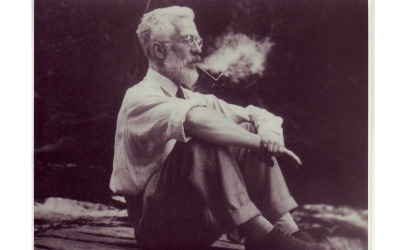
\includegraphics[width=0.8\linewidth]{figs/fisher} \end{figure}
\end{column}
\end{columns}
\end{frame}

\begin{frame}{What is Significance?}
\phantomsection\label{what-is-significance}
\begin{itemize}
\item
  A statistical result is \textbf{significant} if it is \textbf{unlikely
  to have occurred by chance}.
\item
  Even though there is natural variability in the population, the
  probability of observing a value this extreme due to random
  variability is \textbf{low} (though not impossible).
\end{itemize}

\begin{itemize}
\tightlist
\item
  We use probabilities (\textbf{p-values}) and an \textbf{alpha
  threshold (commonly 0.05)} to determine whether a result is
  significant.
\end{itemize}
\end{frame}

\begin{frame}{What is Significance?}
\phantomsection\label{what-is-significance-1}
\begin{itemize}
\tightlist
\item
  Significance refers to the risk of rejecting the null hypothesis when
  it is actually true.
\end{itemize}

\begin{itemize}
\tightlist
\item
  It tells us the probability that our result happened by chance alone.
\end{itemize}

\begin{itemize}
\tightlist
\item
  A p-value of 0.05 (5\%) means there's a 5\% chance the result is due
  to random chance.
\end{itemize}

\begin{itemize}
\tightlist
\item
  A p-value of 0.01 (1\%) means there's a 1\% chance the result happened
  by chance.
\end{itemize}
\end{frame}

\begin{frame}{Calculating Significance}
\phantomsection\label{calculating-significance}
\begin{itemize}
\item
  To quantify a probability, you first need to calculate a \textbf{test
  statistic} and locate it on the normal probability curve.
\item
  The normal curve acts as a statistical translator.

  \begin{itemize}
  \tightlist
  \item
    It helps you standardize your test statistic to a common scale.
  \item
    This standardized value is then used to determine the probability of
    obtaining such a result in a standard normal population.
  \end{itemize}
\end{itemize}
\end{frame}

\begin{frame}{Z-score}
\phantomsection\label{z-score}
\begin{itemize}
\tightlist
\item
  \textbf{Z-scores} link measured or hypothesized values to
  probabilities.
\end{itemize}

\begin{itemize}
\tightlist
\item
  A Z-score (or standard score) indicates how many standard deviations a
  value \emph{\emph{x}} is above or below the mean on the normal curve.
\end{itemize}

\begin{itemize}
\item
  It helps standardize values and connect them to probabilities.
\item
  The Z-score is calculated using the formula:
\end{itemize}

\[ Z = \frac{(x - \mu)}{\sigma} \]

\begin{itemize}
\tightlist
\item
  where:

  \begin{itemize}
  \tightlist
  \item
    \(x\) = the value of interest.\\
  \item
    \(\mu\) = mean of the population.\\
  \item
    \(\sigma\) = standard deviation of the population.
  \end{itemize}
\end{itemize}
\end{frame}

\begin{frame}{Z-Scores: Linking Observations to Probabilities}
\phantomsection\label{z-scores-linking-observations-to-probabilities}
\begin{itemize}
\tightlist
\item
  \textbf{Z-scores} link observations to probabilities.
\item
  Using a Z-score for probability:

  \begin{itemize}
  \tightlist
  \item
    Z-scores are essentially the \textbf{x-axis} of the standard normal
    distribution.
  \item
    They normalize any data set so that the mean is 0 and the standard
    deviation is 1.
  \item
    The area under the curve tells you the probability of a certain
    Z-score occurring.
  \item
    By using the Z-score, we can determine the probability associated
    with different values.
  \end{itemize}
\end{itemize}
\end{frame}

\begin{frame}{Finding Probabilities for Z-Scores}
\phantomsection\label{finding-probabilities-for-z-scores}
\begin{columns}[T]
\begin{column}{0.48\textwidth}
\vspace{1cm}

\begin{itemize}
\tightlist
\item
  \textbf{P(X \textless{} z)}: Denotes the probability of a value
  falling \textbf{less than} a given Z-score (\(z\)).
\end{itemize}

\vspace{1cm}

\begin{itemize}
\tightlist
\item
  \textbf{P(X \textgreater{} z)}: Denotes the probability of a value
  falling \textbf{above} a given Z-score (\(z\)).
\end{itemize}

\vspace{1cm}

\begin{itemize}
\tightlist
\item
  \textbf{P(z1 \textless{} X \textless{} z2)}: Denotes the probability
  of a value falling \textbf{between} two different Z-scores (\(z1\) and
  \(z2\)).
\end{itemize}
\end{column}

\begin{column}{0.48\textwidth}
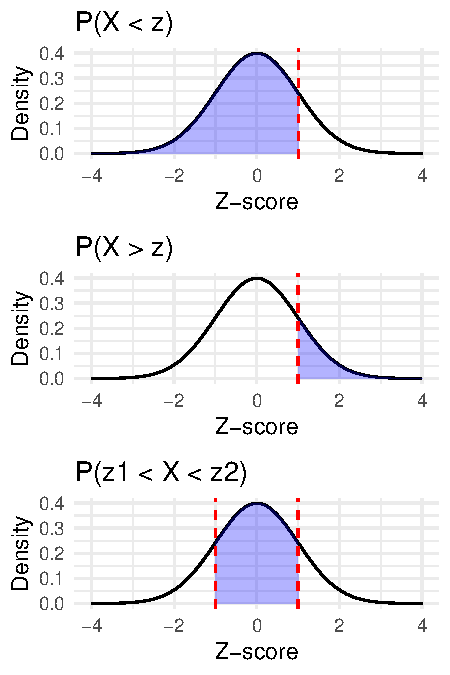
\includegraphics{M5-Hypothesis-Testing,-Probability-and-Distributions_files/figure-beamer/unnamed-chunk-2-1.pdf}
\end{column}
\end{columns}
\end{frame}

\begin{frame}{Example}
\phantomsection\label{example}
\end{frame}

\begin{frame}{Example: Probability of a Cat Living to a Certain Age}
\phantomsection\label{example-probability-of-a-cat-living-to-a-certain-age}
\begin{itemize}
\tightlist
\item
  The lifespan of domestic cats is normally distributed with a mean of
  15.7 years and a standard deviation of 1.6 years.
\end{itemize}

\begin{columns}[T]
\begin{column}{0.48\textwidth}
\vspace{1cm}

\begin{itemize}
\tightlist
\item
  \textbf{Question}: What is the probability that a cat will live to be
  as old as Allison's 18-year-old cat?
\end{itemize}

\begin{itemize}
\tightlist
\item
  We're looking for the probability P(X \textgreater{} 18), which
  represents the probability that a cat will live longer than 18 years.
\end{itemize}
\end{column}

\begin{column}{0.48\textwidth}
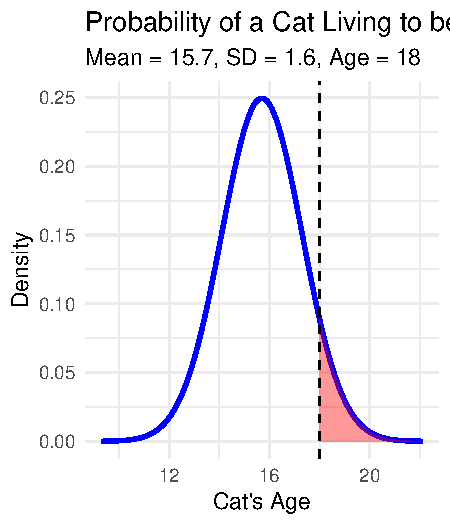
\includegraphics{M5-Hypothesis-Testing,-Probability-and-Distributions_files/figure-beamer/unnamed-chunk-3-1.pdf}
\end{column}
\end{columns}
\end{frame}

\begin{frame}{\textbf{Steps 1}:}
\phantomsection\label{steps-1}
\begin{itemize}
\tightlist
\item
  \textbf{Calculate the Z-score}:
\end{itemize}

\begin{columns}[T]
\begin{column}{0.48\textwidth}
\[
   Z = \frac{X - \mu}{\sigma}
   \]

\begin{itemize}
\tightlist
\item
  where:

  \begin{itemize}
  \tightlist
  \item
    \(X\) is the value (18 years),
  \item
    \(\mu\) is the mean (15.7 years),
  \item
    \(\sigma\) is the standard deviation (1.6 years).
  \end{itemize}
\end{itemize}
\end{column}

\begin{column}{0.48\textwidth}
\vspace{1cm}

\[
   Z = \frac{18 - 15.7}{1.6} = \frac{2.3}{1.6} \approx 1.4375
   \]
\end{column}
\end{columns}
\end{frame}

\begin{frame}[fragile]{Step 2.}
\phantomsection\label{step-2.}
\begin{itemize}
\tightlist
\item
  Find the Probability:
\end{itemize}

\begin{Shaded}
\begin{Highlighting}[]
\CommentTok{\# Given values}
\NormalTok{mean\_lifespan }\OtherTok{\textless{}{-}} \FloatTok{15.7}
\NormalTok{sd\_lifespan }\OtherTok{\textless{}{-}} \FloatTok{1.6}
\NormalTok{age\_allison\_cat }\OtherTok{\textless{}{-}} \DecValTok{18}
\CommentTok{\# Calculate Z{-}score}
\NormalTok{z\_score }\OtherTok{\textless{}{-}}\NormalTok{ (age\_allison\_cat }\SpecialCharTok{{-}}\NormalTok{ mean\_lifespan) }\SpecialCharTok{/}\NormalTok{ sd\_lifespan}
\CommentTok{\# Find the probability that a cat lives longer than 18 years}
\NormalTok{probability }\OtherTok{\textless{}{-}} \DecValTok{1} \SpecialCharTok{{-}} \FunctionTok{pnorm}\NormalTok{(z\_score)}
\NormalTok{probability}
\end{Highlighting}
\end{Shaded}

\begin{verbatim}
## [1] 0.07528799
\end{verbatim}

\begin{itemize}
\tightlist
\item
  Thus, the probability that a cat will live to be as old as or older
  than 18 years is approximately \textbf{0.0749} or \textbf{7.49\%}.
\end{itemize}
\end{frame}

\begin{frame}[fragile]{Step 2.}
\phantomsection\label{step-2.-1}
\begin{itemize}
\tightlist
\item
  Find the Probability:
\end{itemize}

\begin{Shaded}
\begin{Highlighting}[]
\CommentTok{\# Given values}
\NormalTok{mean\_lifespan }\OtherTok{\textless{}{-}} \FloatTok{15.7}
\NormalTok{sd\_lifespan }\OtherTok{\textless{}{-}} \FloatTok{1.6}
\NormalTok{age\_allison\_cat }\OtherTok{\textless{}{-}} \DecValTok{18}
\CommentTok{\# Calculate Z{-}score}
\NormalTok{z\_score }\OtherTok{\textless{}{-}}\NormalTok{ (age\_allison\_cat }\SpecialCharTok{{-}}\NormalTok{ mean\_lifespan) }\SpecialCharTok{/}\NormalTok{ sd\_lifespan}
\CommentTok{\# Find the probability that a cat lives longer than 18 years}
\NormalTok{probability }\OtherTok{\textless{}{-}} \DecValTok{1} \SpecialCharTok{{-}} \FunctionTok{pnorm}\NormalTok{(z\_score)}
\NormalTok{probability}
\end{Highlighting}
\end{Shaded}

\begin{verbatim}
## [1] 0.07528799
\end{verbatim}

\begin{itemize}
\tightlist
\item
  This example walks you through calculating the probability in R using
  \texttt{pnorm()}, which calculates the cumulative probability under
  the normal distribution.
\end{itemize}
\end{frame}

\begin{frame}{What is a P-Value?}
\phantomsection\label{what-is-a-p-value}
\begin{itemize}
\tightlist
\item
  \textbf{Definition}: The p-value is the probability of obtaining a
  result at least as extreme as the one observed, assuming the null
  hypothesis is true.
\end{itemize}

\begin{itemize}
\tightlist
\item
  In Simple Terms, it tells us how likely it is to see the data we have
  (or something more extreme) if there were actually no effect or
  difference.
\end{itemize}

\begin{itemize}
\item
  Interpretation:

  \begin{itemize}
  \tightlist
  \item
    A small p-value indicates that the observed result is unlikely under
    the null hypothesis, suggesting evidence against it.
  \end{itemize}
\end{itemize}

\begin{itemize}
\tightlist
\item
  A large p-value suggests that the observed result is consistent with
  the null hypothesis.
\end{itemize}
\end{frame}

\begin{frame}{}
\phantomsection\label{section}
\end{frame}

\begin{frame}{Hypothesis Testing Summary}
\phantomsection\label{hypothesis-testing-summary}
\begin{longtable}[]{@{}
  >{\raggedright\arraybackslash}p{(\columnwidth - 4\tabcolsep) * \real{0.1890}}
  >{\raggedright\arraybackslash}p{(\columnwidth - 4\tabcolsep) * \real{0.3963}}
  >{\raggedright\arraybackslash}p{(\columnwidth - 4\tabcolsep) * \real{0.4146}}@{}}
\toprule\noalign{}
\begin{minipage}[b]{\linewidth}\raggedright
Scenario
\end{minipage} & \begin{minipage}[b]{\linewidth}\raggedright
Null Hypothesis is True
\end{minipage} & \begin{minipage}[b]{\linewidth}\raggedright
Null Hypothesis is False
\end{minipage} \\
\midrule\noalign{}
\endhead
\textbf{Reject Null Hypothesis} & \textbf{Type I Error}: Incorrectly
rejecting the null hypothesis. & \textbf{Correct Decision}: Correctly
rejecting the null hypothesis. \\
\textbf{Fail to Reject Null Hypothesis} & \textbf{Correct Decision}:
Correctly not rejecting the null hypothesis. & \textbf{Type II Error}:
Incorrectly failing to reject the null hypothesis. \\
\bottomrule\noalign{}
\end{longtable}
\end{frame}

\begin{frame}{Hypothesis Testing Summary}
\phantomsection\label{hypothesis-testing-summary-1}
\begin{longtable}[]{@{}
  >{\raggedright\arraybackslash}p{(\columnwidth - 4\tabcolsep) * \real{0.1890}}
  >{\raggedright\arraybackslash}p{(\columnwidth - 4\tabcolsep) * \real{0.3963}}
  >{\raggedright\arraybackslash}p{(\columnwidth - 4\tabcolsep) * \real{0.4146}}@{}}
\toprule\noalign{}
\begin{minipage}[b]{\linewidth}\raggedright
Scenario
\end{minipage} & \begin{minipage}[b]{\linewidth}\raggedright
Null Hypothesis is True
\end{minipage} & \begin{minipage}[b]{\linewidth}\raggedright
Null Hypothesis is False
\end{minipage} \\
\midrule\noalign{}
\endhead
\textbf{Reject Null Hypothesis} & \textbf{Type I Error}: Incorrectly
rejecting the null hypothesis. & \textbf{Correct Decision}: Correctly
rejecting the null hypothesis. \\
\textbf{Fail to Reject Null Hypothesis} & \textbf{Correct Decision}:
Correctly not rejecting the null hypothesis. & \textbf{Type II Error}:
Incorrectly failing to reject the null hypothesis. \\
\bottomrule\noalign{}
\end{longtable}

\small - Failing to reject the null hypothesis means our data didn't
show a significant effect. It doesn't prove the null hypothesis is true;
it just means we didn't find strong evidence against it.\\
\end{frame}

\begin{frame}{}
\phantomsection\label{section-1}
\begin{itemize}
\item
  \textbf{Explanation}:

  \begin{itemize}
  \tightlist
  \item
    \textbf{Type I Error}: False positive. We conclude there is an
    effect or difference when there is none.
  \end{itemize}
\end{itemize}

\begin{itemize}
\tightlist
\item
  \textbf{Type II Error}: False negative. We fail to detect an effect or
  difference when one exists.
\end{itemize}

\begin{itemize}
\tightlist
\item
  \textbf{Correct Decisions}: Accurately concluding the presence or
  absence of an effect or difference based on the truth of the null
  hypothesis.
\end{itemize}
\end{frame}

\begin{frame}{}
\phantomsection\label{section-2}
\end{frame}

\end{document}
